\section{\uppercase{Experiments and Results}}
\label{sec:experiments}

% RQ1 from PAPER_FACTS section 11, RQ2 from sections 9-10 (B200), RQ3 from section 13 (L40S).

Unless stated otherwise, ``TEST'' denotes the 73-image test split (1{,}210 species instances) and ``VAL'' the 52-image validation split; species metrics follow the fixed-threshold protocol of Section~\ref{sec:method:protocol} (score$\ge$0.25, IoU$\ge$0.5, micro-averaged over the four species). In Sections~\ref{sec:exp:rq2v9} and~\ref{sec:exp:rq3} detectors are trained with seeds 0--2 and cascade classifiers with seeds 42, 84 and 126 (the nine detector--classifier pairs of a configuration are crossed, not independent); values are mean$\pm$std over seeds and deltas are mean$\pm$std of paired differences (Section~\ref{sec:method:protocol}). Section~\ref{sec:exp:rq1} uses seeds 0--2 on the same TEST.

\subsection{RQ1: Effect of Targeted Collections}
\label{sec:exp:rq1}

RQ1 asks whether the targeted collections of Section~\ref{sec:dataset:collections} improve species-level detection, in the scenarios they address, and whether species confusion also changes. We distinguish finding an insect (localization) from finding it and assigning the correct species.

\paragraph{Hypotheses.}
The initial hypotheses, recorded before the runs, were: \textbf{H1}, the collections improve species recall for small specimens and crowded plates and reduce species false positives on insect-only plates; \textbf{H2}, confusion between species, particularly MC$\leftrightarrow$MV, is unchanged among localized objects.

\paragraph{Training sets.}
Since v4 is not a subset of DS-F2\_v9.0.5, training sets are built from plate batches: \textbf{L0}, v5.1 (103 training images); \textbf{L1}, L0 plus v6.0 and v7 (244); \textbf{L2}, L1 plus v8 and v9, without copy-paste (869). Two alternative extensions of L2: \textbf{L2+ORG} adds white-paper photographs (1{,}497 images); \textbf{L3}, the full v9.0.5 training split, adds copy-paste and no DS-ORG (1{,}738; it reuses the E0 runs of Section~\ref{sec:exp:rq2v9}). Counts include augmented images. To separate quantity from targeting, we add an equal-size control: random subsamples of the L3 training split with the size of L1 (244 images, three seeds) and of L2 (869 images, three seeds), each drawn with the seed of its run. All arms use the E0 recipe of Section~\ref{sec:method:single} with seeds 0--2 and the metrics of Section~\ref{sec:method:protocol}. Differences against L3 carry a 95\% bootstrap CI over test images (10{,}000 resamples, seeds pooled) and an exact McNemar test per seed. Size bins on $\sqrt{wh}$: $<$32, 32--48, $\ge$48\,px; a plate is crowded at $\ge$30 species instances (7 TEST plates); 6 contain only INS.

\paragraph{H1: detection improves where the collections aim.}
Table~\ref{tab:rq1_ablation} gives the ladder. Overall species recall rises monotonically, $0.561\pm0.006$ (L0), $0.738\pm0.004$ (L1), $0.797\pm0.015$ (L2), $0.811\pm0.012$ (L2+ORG), $0.822\pm0.016$ (L3), and localization recall (class ignored) rises from 0.923 to 0.977. Recall on objects below 32\,px goes from 44\% to 81\%, and species false positives on the six insect-only plates fall from 66--87 (L0) and 43--57 (L1) per seed to 0 in L2 and L3 (at most 3 in L2+ORG). Recall on crowded plates goes from 59\% to 84\%. Against L3, L0 and L1 are worse ($\Delta=-0.261$ [$-0.335$, $-0.189$] and $-0.084$ [$-0.123$, $-0.049$]). L2 is $-0.025$ [$-0.048$, $-0.001$] and L2+ORG is $-0.012$ [$-0.029$, $+0.003$]: the last two steps are at most small. MD recall, the weakest species, stays at 0.64--0.69 from L1 on (std up to 0.11).

\begin{table}[t]
\centering
\caption{RQ1, TEST (73 images, 1{,}210 target instances): YOLO26m, identical recipe, mean$\pm$sample std over seeds 0--2; VAL selects \texttt{best.pt}. Species recall requires localization and the correct class (IoU$\ge$0.5, score$\ge$0.25); localization recall ignores the class. Training counts include augmentations and all seven classes. FP: total target-species predictions on the six INS-only plates, averaged over seeds. Confusion rates: percentages among localized instances of the annotated class, seeds pooled. $\Delta$: overall species recall minus L3, with 95\% image-bootstrap CI.}
\label{tab:rq1_ablation}
\footnotesize
\setlength{\tabcolsep}{2.5pt}
\resizebox{\linewidth}{!}{%
\begin{tabular}{@{}lrrrrr@{}}
\toprule
 & L0 & L1 & L2 & L2+ORG & L3 \\
\midrule
Train images / boxes (k) & 103 / 4.4 & 244 / 10.6 & 869 / 33.1 & 1497 / 69.3 & 1738 / 88.1 \\
\midrule
\multicolumn{6}{@{}l}{\emph{Overall performance and targeted scenarios}} \\
Overall species recall (\%) & 56.1$\pm$0.6 & 73.8$\pm$0.4 & 79.7$\pm$1.5 & 81.1$\pm$1.2 & 82.2$\pm$1.6 \\
$\Delta$ vs.\ L3 (pp) & $-26.1$ & $-8.4$ & $-2.5$ & $-1.2$ & --- \\
\quad 95\% CI & [$-33.5$, $-18.9$] & [$-12.3$, $-4.9$] & [$-4.8$, $-0.1$] & [$-2.9$, $+0.3$] & --- \\
Localization recall (\%) & 92.3$\pm$1.7 & 96.0$\pm$0.6 & 97.6$\pm$0.3 & 97.9$\pm$0.2 & 97.7$\pm$0.4 \\
Species recall $<$32\,px (\%) & 44.2$\pm$1.1 & 71.8$\pm$3.7 & 76.5$\pm$4.3 & 78.8$\pm$2.8 & 80.5$\pm$0.7 \\
Species recall 32--48\,px (\%) & 62.9$\pm$5.3 & 71.7$\pm$3.6 & 79.3$\pm$2.5 & 79.7$\pm$2.6 & 80.2$\pm$2.6 \\
Species recall $\ge$48\,px (\%) & 77.4$\pm$9.7 & 83.1$\pm$3.8 & 89.6$\pm$0.9 & 89.4$\pm$1.5 & 90.5$\pm$3.2 \\
Species recall, crowded plates (\%) & 58.7$\pm$0.4 & 75.6$\pm$1.5 & 78.8$\pm$5.5 & 82.8$\pm$2.6 & 83.8$\pm$2.2 \\
Species FP, INS-only plates (mean) & 75.7 & 48.3 & 0 & 1.7 & 0 \\
\midrule
\multicolumn{6}{@{}l}{\emph{Species confusion among localized instances}} \\
MC$\to$MV, localized (\%) & 18.5 & 19.1 & 14.5 & 15.0 & 11.7 \\
MV$\to$MC, localized (\%) & 14.8 & 8.0 & 6.3 & 6.3 & 5.4 \\
\bottomrule
\end{tabular}%
}
\end{table}

\paragraph{Quantity versus targeting.}
Random subsamples of L3 reach species recall $0.752\pm0.077$ at 244 images (L1: $0.738\pm0.004$) and $0.800\pm0.007$ at 869 images (L2: $0.797\pm0.015$), three seeds each. The targeted sets are thus indistinguishable from random subsets of the final data: up to L2 the rise is mostly the number of images (244-image subsamples vary from 0.69 to 0.84 across seeds, so only a large effect would be visible). At 103 images the picture reverses: a random subsample of L3 reaches $0.754\pm0.007$, 19\,pp above L0 ($0.561$). The L0 deficit is thus not only quantity; the control cannot separate label quality from version.

\paragraph{Changes in species confusion (H2).}
Figure~\ref{fig:rq1_confusion} compares L0 and L3 among localized instances. MV$\to$MC confusion decreases from 14.8\% to 5.4\%, MC$\to$MV from 18.5\% to 11.7\%, and the share of localized MF assigned to a non-target class from 46\% to 9\%; no MF$\leftrightarrow$MC confusion is observed in any arm. The pattern is a reduction in these rates rather than the unchanged identification anticipated by H2, but residual confusion remains, particularly MC$\to$MV at 11.7\% in L3. The rates pool the three seeds and use the objects localized by each model as denominators; they are point estimates without intervals.
% TODO(TEAM): do we have confidence intervals or variability measures for the confusion-rate differences?

\begin{figure}[t]
\centering
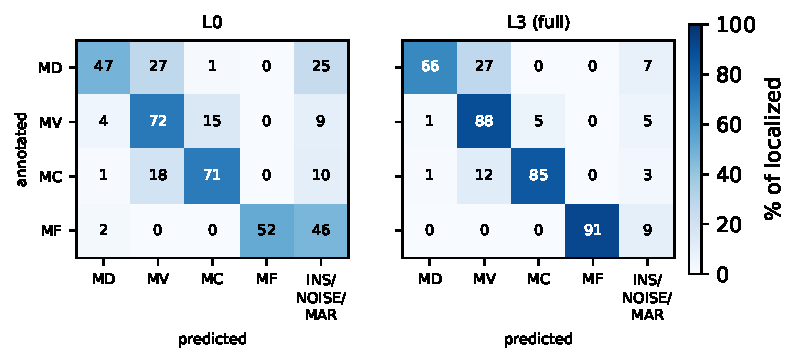
\includegraphics[width=0.55\linewidth]{figs/rq1_confusion.pdf}
\caption{RQ1, TEST: confusion among localized target instances for L0 (left) and L3 (right), seeds 0--2 pooled; each row is a percentage of localized instances of the annotated class (missed instances excluded; right block: predicted INS, NOISE or MAR).}
\label{fig:rq1_confusion}
\end{figure}

\paragraph{Scope.}
Size and composition vary together, so the comparisons give combined effects. L0 has 103 images; DS-ORG is about 42\% of L2+ORG, and L2+ORG and L3 are alternative extensions of L2, so their difference does not isolate copy-paste. One fixed TEST split and three seeds; the crowded (7) and INS-only (6) subsets are descriptive.


\subsection{RQ2 on DS-F2\_v9.0.5: Cascade, Oracle and the Identification Ceiling}
\label{sec:exp:rq2v9}


\paragraph{Setup.} VAL selected \texttt{best.pt}, so VAL numbers are not held out and serve only as a consistency check. Metrics are macro-F1 over the four species at score$\ge$0.25 and IoU$\ge$0.5. Stage~2 is a ConvNeXt-T~\cite{liu2022convnext} (CE or part-aware head), DINOv2, DINOv3 or BioCLIP~2, all fully fine-tuned. Detectors: E0 (three seeds), YOLO26l (one seed), RT-DETR-l~\cite{zhao2024rtdetr} (three seeds). Intervals are 95\% BCa bootstrap over test images (10{,}000 resamples, paired with the detector-only run) with a sign-flip permutation test~\cite{du2025pairedbootstrap}.

\paragraph{The cascade does not improve on the detector.} On TEST, E0 alone reaches 79.5\% macro-F1 and every one of the five stage-2 backbones lowers it: $\Delta$F1 is $-2.7$ [$-4.8$, $-0.3$] pp for ConvNeXt-T CE ($p_{\text{perm}}=0.013$), $-1.4$ [$-3.7$, $+1.3$] for parts, $-1.7$ [$-3.5$, $+0.1$] for DINOv2, $-2.0$ [$-4.0$, $+0.3$] for DINOv3 and $-1.1$ [$-2.7$, $+0.8$] for BioCLIP~2 (E0, nine pairs). With YOLO26l (80.5\%) the shifts are $-2.1$ to $-4.0$ pp, and with RT-DETR-l (74.6\%) $-2.3$ to $-5.1$ pp. Single-configuration intervals often include zero (73 images), but the sign is the same in all 5$\times$3 configurations (YOLO26l has one seed); McNemar $p$ varies between seeds ($0.005$--$0.51$ for CE with E0), so we do not summarize it.

\paragraph{Why: a ceiling at identification.} With ground-truth crops the classifiers reach 82.7--83.8\% species accuracy on TEST (87--88\% on VAL), regardless of backbone family; a better backbone does not lift the ceiling. This is a plateau, not a proven information limit: the detector alone is at $\approx$84\% among localized objects (82.2/97.7). Across the 15 classifiers, 60.0\% of instances are correct for all and 4.9\% are wrong for all; majority vote gives 86.3\% against a mean of 83.4\%. Errors are confident (69.4\% have max-softmax $\ge0.8$) and concentrated in the MD/MV/MC family (family-level accuracy 96.0\% vs.\ 80.6\% by species). Abstention (keeping the detector label below a confidence $\tau$) gains at most $+0.2$\,pp. Confident learning flags 3.7\% (127/3{,}470) of the TEST crops and 4.1\% of VAL as suspect labels, mostly NOISE$\leftrightarrow$MF, MD$\leftrightarrow$MV and MC$\leftrightarrow$MV; we have no expert review, so ``suspect'' does not mean ``wrong''. The rate is in the range reported for curated benchmarks~\cite{northcutt2021pervasive}.

\paragraph{Limitations and open items.} No expert re-labelled the confusable pairs, so ambiguity cannot be separated from label noise. A near-duplicate check finds no VAL or TEST image with thumbnail similarity $\ge0.98$ to a training image, but 4.7\% of TEST crops reach it against some training crop (plausibly glue background), so we do not claim absence of leakage at crop level. \paragraph{Background class.} A natural fix for the species that the seven-way head sends to \emph{non-species} is an eight-way head with an explicit background class trained on detector false positives (BG). With three classifier seeds on the E0 detectors, BG gives $\Delta$F1 $-2.8$ [$-4.8$, $-0.4$] pp on TEST ($p_{\text{perm}}=0.010$) and $-5.4$ pp on VAL, the same as the CE control ($-2.7$ and $-5.5$ pp); its accuracy on ground-truth crops is $77.6\pm2.8$\% (TEST), not higher. The background class does not remove the loss. Oracle accuracy with 25\%, 50\% and 100\% of the training crops (ConvNeXt-T, one seed) is flat on TEST (83.0, 81.7, 82.6\%), compatible with ambiguity but not proof of it.

\begin{table}[t]
\centering
\caption{Per-species TEST results, E0 alone vs.\ the ConvNeXt-T CE cascade (mean of nine pairs; recall, precision and F1 in \%; count error = mean $|n_{\text{pred}}-n_{\text{GT}}|$ per image).}
\label{tab:persp}
\footnotesize
\setlength{\tabcolsep}{3pt}
\begin{tabular}{@{}lrrrrrrrr@{}}
\toprule
 & \multicolumn{4}{c}{E0 alone} & \multicolumn{4}{c}{Cascade} \\
\cmidrule(r){2-5}\cmidrule(l){6-9}
 & R & P & F1 & err & R & P & F1 & err \\
\midrule
MD & 64.9 & 78.8 & 71.2 & 1.17 & 61.4 & 70.4 & 65.5 & 1.49 \\
MV & 87.9 & 69.0 & 77.3 & 1.67 & 85.6 & 68.8 & 76.2 & 1.96 \\
MC & 84.6 & 86.1 & 85.3 & 0.76 & 84.3 & 86.3 & 85.3 & 0.78 \\
MF & 86.0 & 82.9 & 84.4 & 0.83 & 87.1 & 74.9 & 80.5 & 1.41 \\
\bottomrule
\end{tabular}
\end{table}

\paragraph{Fusion, margin, cost and localization.} The detector exposes only its top-1 class and score, so a fusion with its full class distribution was not run. On TEST, F1 (nine pairs) is 79.5\% for E0, 76.9\% for the cascade and 79.6\% for a soft fusion, which only matches the detector. Two variants of the ConvNeXt-T CE cascade (species accuracy on TEST, H100) do not change the picture: relabelling only the proposals called a species gives $-1.5$ [$-3.2$, $+0.3$] pp against the detector alone, and a late fusion with its top-1 score (weight chosen on VAL) $+0.3$ [$-0.1$, $+0.7$] pp; on the B200 the same fusion gave $+1.3$ pp, so we read it as hardware-dependent noise. Retraining the classifier with a smaller context margin makes the cascade worse: $-0.9$ pp at 75\% of the box per side (paper setting), $-2.8$ [$-5.0$, $-0.3$] at 25\% and $-2.5$ [$-5.3$, $+0.6$] at 0\%. These runs use another GPU than the main table (detector alone differs by 0.6 pp), so margins are compared only among themselves. E0 localizes $97.7\pm0.4$\% of the TEST species instances (RT-DETR 98.5\%), so the remaining error is identification.

\subsection{RQ3: Transfer of Tiny-Object Methods}
\label{sec:exp:rq3}

\paragraph{Protocol.}
RQ3 was run as a separate campaign on a different GPU (L40S) with the same recipe as E0 (YOLO26m, 150 epochs, batch 8, \texttt{imgsz} 1920, patience 30) and the same data, so its own E0 (three seeds) is the only control for the variants below; we do not mix it with the E0 of other tables. The variants are: NWD ($w{=}0.5$, $C{=}44$\,px) in the loss only, NWD in the assigner only, NWD plus RFLA, the scale-adaptive GCD ($w{=}0.5$), Wise-IoU v3, a P2 head, training and inference at \texttt{imgsz} 2560 (batch 4), and, with one seed, YOLO11m. The metric is species accuracy on TEST: a ground-truth species instance counts as correct if a detection with score $\ge0.25$ matches it at IoU$\ge$0.5 and has the right class (equal to micro recall over the 1{,}210 species instances). $\Delta$ is the per-seed difference to E0 of the same seed, with a 95\% bootstrap interval over images (10{,}000 resamples), and $p$ is Holm-corrected over the eight comparisons.

\paragraph{No variant improves on E0.}
Table~\ref{tab:rq3_main} shows that no variant has a positive $\Delta$ whose interval excludes zero. GCD, Wise-IoU v3 and NWD in the assigner only are indistinguishable from E0 ($\Delta$ between $-0.3$ and $+0.3$\,pp); their intervals are $\approx\pm1.7$\,pp wide, so we claim no difference detected, not equivalence. P2, \texttt{imgsz} 2560 and NWD in the loss only are $2.5$--$3.8$\,pp below E0 and do not survive the Holm correction ($p=0.14$, 0.057, 0.084). Only NWD+RFLA is $8.8$\,pp below E0 (Holm $p=0.002$) and unstable: one seed stopped early at epoch~40 with its best epoch near~10, and another diverged (classification loss in the thousands from epoch~27, \texttt{nan} at epoch~30); we kept the recipe and did not retry, so the mean of $72.9\pm7.5$\% includes both. NWD acts through its loss, not through the assigner: the assigner-only variant equals E0 while the loss-only variant is $2.5$\,pp lower. YOLO11m (one seed, exploratory) is $1.2$\,pp below, interval including zero.

\begin{table}[t]
\centering
\caption{RQ3 on TEST (73 images, 1{,}210 species instances), YOLO26m, L40S campaign; three seeds unless noted. Accuracy: mean$\pm$std. $\Delta$: paired difference to E0 of the same seed in pp, with 95\% bootstrap interval over images; $p$: Holm over the eight three-seed variants (YOLO11m, one seed, is outside the family; its $p$ is not corrected). Recall (\%) by object size $\sqrt{wh}$ ($n=613$, 376, 221). VAL selected \texttt{best.pt} and is not held out; all numbers are TEST.}
\label{tab:rq3_main}
\footnotesize
\setlength{\tabcolsep}{2.5pt}
\resizebox{\linewidth}{!}{%
\begin{tabular}{@{}lrrrrrr@{}}
\toprule
 & Acc. (\%) & $\Delta$ [95\% CI] & $p$ & $<$32 & 32--48 & $\ge$48 \\
\midrule
E0 (CIoU) & 81.7$\pm$1.2 & --- & --- & 79.4 & 81.0 & 89.4 \\
GCD & 81.5$\pm$0.4 & $-0.2$ [$-1.8$, $+1.6$] & 1.00 & 78.3 & 80.5 & 92.3 \\
Wise-IoU v3 & 81.4$\pm$1.0 & $-0.3$ [$-1.9$, $+1.5$] & 1.00 & 78.9 & 79.6 & 91.4 \\
NWD, assigner only & 82.0$\pm$1.9 & $+0.3$ [$-1.4$, $+2.4$] & 1.00 & 79.4 & 80.6 & 91.7 \\
NWD, loss only & 79.3$\pm$3.4 & $-2.5$ [$-4.5$, $-0.5$] & 0.084 & 74.0 & 80.8 & 91.3 \\
P2 head & 79.0$\pm$2.7 & $-2.8$ [$-5.0$, $-0.4$] & 0.14 & 74.0 & 80.1 & 91.0 \\
\texttt{imgsz} 2560 & 78.0$\pm$3.3 & $-3.8$ [$-6.1$, $-1.1$] & 0.057 & 72.8 & 79.3 & 90.0 \\
NWD + RFLA & 72.9$\pm$7.5 & $\mathbf{-8.8}$ [$-12.7$, $-4.9$] & 0.002 & 63.3 & 78.5 & 90.0 \\
\midrule
YOLO11m (1 seed) & 81.0 & $-1.2$ [$-4.4$, $+2.1$] & --- & 76.3 & 83.0 & 90.5 \\
\bottomrule
\end{tabular}%
}
\end{table}

\paragraph{Tuned NWD against a same-GPU control.}
We also trained NWD (loss and assigner) with other constants on the H100, with its own E0 control (three seeds, $82.2\pm1.9$\%). $w{=}0.5$, $C{=}22$\,px gives $81.7\pm1.5$\% ($-0.5$ [$-2.7$, $+1.8$] pp); $w{=}1.0$, $C{=}44$\,px collapses to $53.9\pm1.3$\% ($-28.3$ [$-34.9$, $-21.4$] pp); $w{=}0.5$, $C{=}88$\,px, with two seeds, gives $81.8\pm3.7$\% ($-0.7$ [$-3.0$, $+1.8$] pp; seeds $-5.2$, $+3.8$). None beats the control.

\paragraph{Recall by object size.}
The smallest objects do not benefit from any variant: the recall below 32\,px is at most equal to E0 (E0 79.4\%, NWD assigner-only 79.4\%) and lower for all others, down to 63.3\% for NWD+RFLA (Table~\ref{tab:rq3_main}). The gains above 48\,px (0.6 to 2.9\,pp) come with a seed spread of 1--5\,pp and are not statistically supported. This agrees with the localization result of RQ2: E0 localizes $97.7\pm0.4$\% of the species instances, so a box-similarity loss has little to repair and the smallest objects are limited by identification.

\paragraph{Sliced inference, test-time augmentation and ensembling.}
We apply three inference-time methods to the three E0 detectors (mAP@50 under a confidence-0.0 evaluator, not the species harness; WBF is a single result over the three seeds). Sliced inference (512\,px tiles, 25\% overlap) reaches a species recall of $86.7\pm1.8$\% and mAP@50 $69.5\pm0.8$, against $35.5\pm0.9$\% and $9.5\pm1.0$ for the same detector run on the whole frame resized to 512\,px. That comparison is unfair (the resize shrinks the frame $\approx$3.75$\times$); the relevant baseline is E0 at native resolution (mAP@50 $84.2\pm0.5$, mAP@50:95 $61.7\pm0.1$), and slicing a detector trained at 1920\,px with 512\,px tiles does not reach it. TTA at 1920 adds $+0.4$ mAP@50 and $+0.5$ mAP@50:95, a small gain. A weighted-boxes-fusion ensemble of the three E0 detectors gives mAP@50 $83.6$, below the single-model mean (84.2), so we find no gain from ensembling either.


\paragraph{Why the aerial loss recipes do not transfer here.}
Three properties of our regime differ from the benchmarks on which NWD, RFLA and SAHI were validated. First, the objects are tiny by the COCO convention but the images are processed at native resolution: a 44-px fly spans about five cells of the stride-8 feature map, whereas the AI-TOD regime for which NWD was designed has objects of a few pixels after the network's own downscaling; the IoU sensitivity that NWD corrects is therefore much milder. Second, YOLO26 already uses a task-aligned dynamic assignment and an NMS-free one-to-one head~\cite{yolo26}; the reported gains of NWD and RFLA come from anchor-based or two-stage detectors with static IoU-threshold assignment~\cite{wang2021nwd,xu2022rfla,xu2022aitod}, where a Gaussian similarity changes which anchors become positive. Third, sliced inference is designed for the case where the alternative is to downscale a large image below the object scale~\cite{akyon2022sahi}; here the detector already runs at native scale. These are untested explanations; $C=44$\,px was measured on an earlier data version.

\subsection{Error Analysis}
\label{sec:exp:errors}

Confusion rates among TEST species for E0 and the E0\,+\,CE cascade (nine detector--classifier pairs, mean; $\Delta$ is mean$\pm$std of the paired difference; MV$\to$non-species 4.7\% to 1.5\%, MC$\to$non-species 3.0\% to 0.7\%). The dominant error of the detector is MD$\rightarrow$MV (26.3\%) and MC$\rightarrow$MV (11.7\%). The cascade moves these only partly: MD$\rightarrow$MV falls by $5.3\pm3.5$\,pp, but the instances do not become correct; MD$\rightarrow$\emph{non-species} rises by $8.0\pm5.1$\,pp (7.0\% to 15.0\%) and MV$\rightarrow$MD rises by $4.9\pm1.2$\,pp (1.4\% to 6.3\%). The seven-way head therefore trades one error for others: MD ends at 61.4\% correct against 64.9\% for the detector. MC$\rightarrow$MV does not move ($+1.4\pm6.2$\,pp). MF is never confused with another species by either system; its errors are non-species and missed objects, which the cascade cannot repair because it does not change boxes (Table~\ref{tab:persp}: recall 86.0\% vs.\ 87.1\%, but precision falls from 82.9\% to 74.9\% as other species are relabelled MF). 



